\documentclass[a4paper, french]{article}
\usepackage{geometry} % permet de redéfinir les marges etc. 
\usepackage{graphicx} % Pour incorporer des grapiques, des couleurs etc.
\usepackage{rotating} % Pour  pivoter du texte
\usepackage{array} % Plus facile pour des tableaux complexes
\usepackage{fontspec}
\usepackage[output-decimal-marker={,}]{siunitx} % indisoensable pour les chiffres avec unité
\usepackage{tikz} % Dessis, graphiques etc.
\usepackage{multirow} %Pour fusionner des cellules sur plusieurs lignes dans les tableaux
\usepackage{longtable} % Pour faire des tableaux sur plusieurs pages
\usepackage{textcomp} % Qelques carctèrs supplémentaires
\usepackage{booktabs} % Fugnloe les lignes horizontales dans les tableaux
\usepackage{xspace} % gère les espaces après des fonctions
\usepackage{babel} % Pour écrire en français
\usepackage{hyperref} % Liens hyper texte inernes & externes
%
\hypersetup{% Réglages des liens hypertextes : couleur etc.
colorlinks=true,
pdftitle={},
pdfauthor={Philippe MICHEL},
pdfkeywords={},
unicode
}
\title{Score d'escarre en réanimation}
\author{Philippe MICHEL}
%
\setmainfont[Mapping=tex-text]
{MinionPro-Regular}
\setsansfont[Mapping=tex-text]
{MyriadPro-Regular}
% Pour avoir une virgule en mode math
\mathcode`\.="013B
%
\newcommand{\pc}[1]{\SI{#1}{\percent}} 
\newcolumntype{C}{>{$}c<{$}} % Colonnes en mode math dans les tableaux
%

\begin{document}
\maketitle

\tableofcontents

\hypertarget{protocole}{%
\section{Protocole}\label{protocole}}

Pour établir un score de gravté il faut disposer de variables toutes
factorielles, idéalement binaires, sinon ordonnées avec peu de valeurs
possibles. Ces variables seront toutes celles parraissant significatives
avec un seuil assez élevé (p \textless{}0,2 par ex.).

Ensuite, sur un premeir groupe de patients pris dns l'échantillon total
 (autour de 1/3) on recherche par régression logistique une formule
simple. Ensite on teste cette frmule sur le reste de l'échantillon voire
unun pseudo échantillon beaucoup plus grand obtenu par bootstrap ou
autre.

\hypertarget{importation-mise-en-forme-des-variables}{%
\section{Importation \& mise en forme des
variables}\label{importation-mise-en-forme-des-variables}}

\hypertarget{facteurs-de-risque-connus}{%
\section{Facteurs de risque connus}\label{facteurs-de-risque-connus}}

Pour mémoire les facteurs de risque d'escarre mis en évidence dans
Pressure sont (en plus de l'IGS II): - Sexe - Alité 7jours avant
l'admission - Poids - Albumine - CRP - Ventilation - Corticoïdes -
maladie neurologique - Type de nutrition

Pour mémoire, en régression, les facteurs retrouvés sont : - Poids
\textgreater{} 90 Kg - Corticoïdes - Maladie neurologique

\hypertarget{recherche-de-seuils}{%
\section{Recherche de seuils}\label{recherche-de-seuils}}

Pour les variables numériques (poids, albumine, CRP), on recherche un
seuil * significatif * par les courbes de ROC.

Malheureusement ces trois variables ont des courbes ROC très plates sans
seuil bien défini. Néanmoins des seuils un peu moins mauvais ont pu être
trouvés : - Poids : 90 Kg - Albumine: 23 - CRP : 90

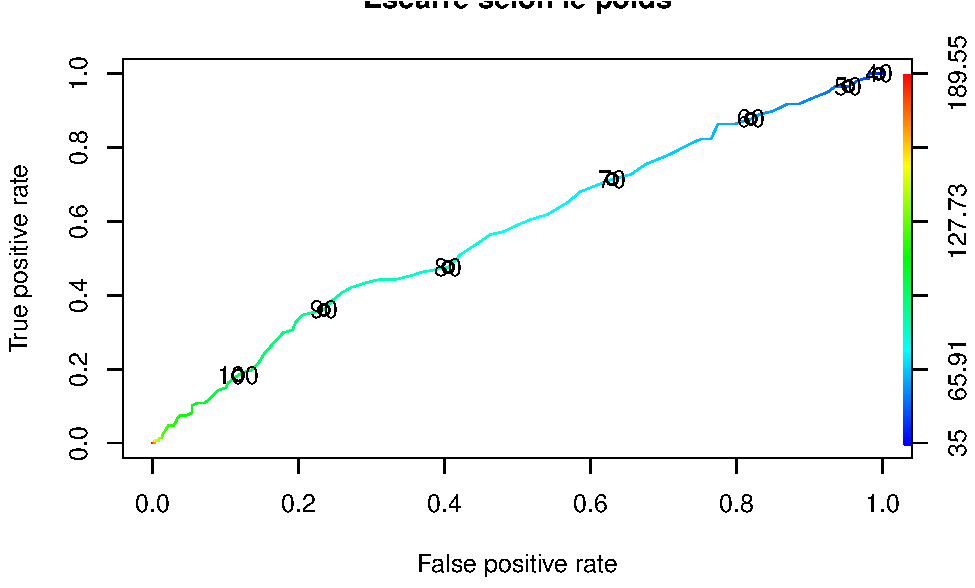
\includegraphics{book_escarre_files/figure-latex/roc-1.pdf}
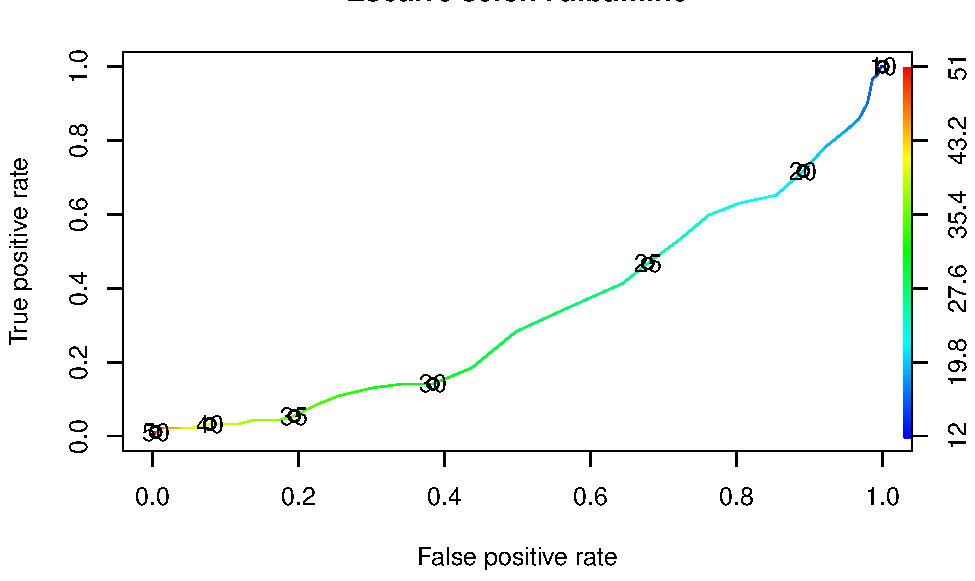
\includegraphics{book_escarre_files/figure-latex/roc-2.pdf}
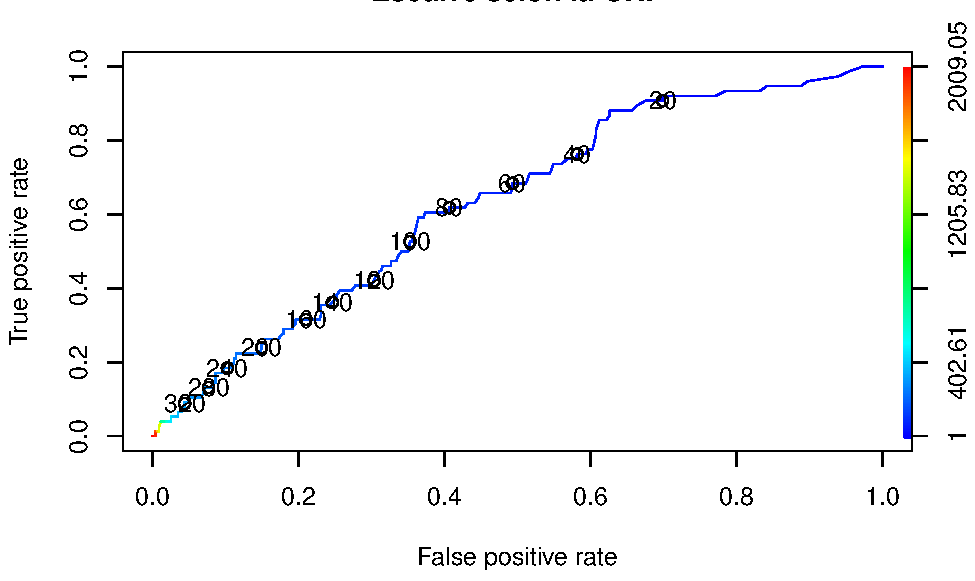
\includegraphics{book_escarre_files/figure-latex/roc-3.pdf}
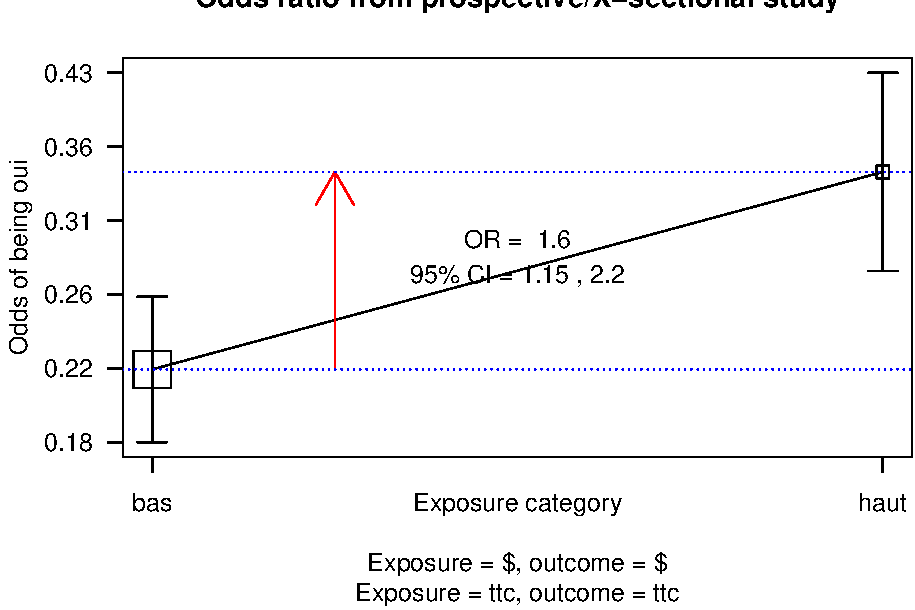
\includegraphics{book_escarre_files/figure-latex/roc-4.pdf}

\begin{verbatim}
## 
##             ttc$poids
## ttc$escarrej  bas haut Total
##        non    729  224   953
##        oui    157   77   234
##        Total  886  301  1187
## 
## OR =  1.6 
## Exact 95% CI =  1.15, 2.2  
## Chi-squared = 8.77, 1 d.f., P value = 0.003
## Fisher's exact test (2-sided) P value = 0.004
\end{verbatim}

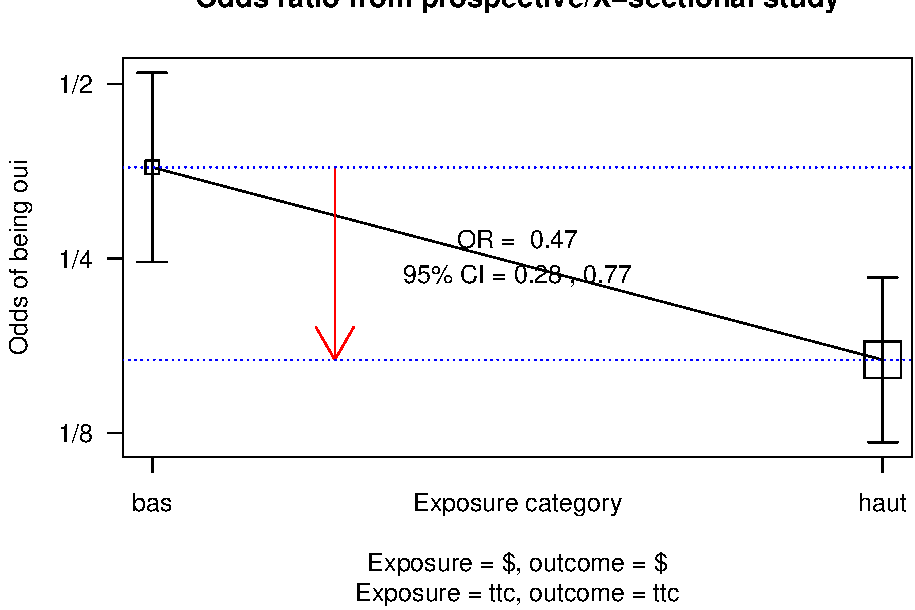
\includegraphics{book_escarre_files/figure-latex/roc-5.pdf}

\begin{verbatim}
## 
##             ttc$albumine
## ttc$escarrej bas haut Total
##        non   106  330   436
##        oui    51   90   141
##        Total 157  420   577
## 
## OR =  0.57 
## Exact 95% CI =  0.37, 0.87  
## Chi-squared = 7.56, 1 d.f., P value = 0.006
## Fisher's exact test (2-sided) P value = 0.009
\end{verbatim}

\begin{verbatim}
## 
##             ttc$crp
## ttc$escarrej bas haut Total
##        non   430    2   432
##        oui   117    0   117
##        Total 547    2   549
## 
## OR =  0 
## Exact 95% CI =  0, 19.71  
## Chi-squared = 0.54, 1 d.f., P value = 0.461
## Fisher's exact test (2-sided) P value = 1
\end{verbatim}

On dispose ainsi de variables factorielles simples, binaires pour tous
les facteurs à étudier

\hypertarget{regression-logistique-preparatoire}{%
\section{Régression logistique
(préparatoire)}\label{regression-logistique-preparatoire}}

Pour ces travaux préparatoires j'utilise tout l'échantillon. Le
protocole complet ne sear utilisé que lorsqu'un score semblera être
meilleur. On lance la régression sur les variables retenues.

\begin{verbatim}
## 
## Call:
## glm(formula = escarrej ~ alite.avant + sexe + poids + albumine + 
##     crp + vent + cort + mal_ad + nut, family = "binomial", data = ttc)
## 
## Deviance Residuals: 
##     Min       1Q   Median       3Q      Max  
## -1.6602  -0.6990  -0.4860  -0.3398   2.3390  
## 
## Coefficients:
##                Estimate Std. Error z value Pr(>|z|)   
## (Intercept)      1.0860     0.5856   1.854  0.06368 . 
## alite.avantnon  -0.8490     0.3223  -2.634  0.00844 **
## sexeH            0.1544     0.3294   0.469  0.63937   
## poidshaut        0.8057     0.3290   2.449  0.01433 * 
## albuminehaut    -0.5346     0.3422  -1.563  0.11816   
## crphaut        -12.7034   882.7435  -0.014  0.98852   
## ventnon         -0.2745     0.4030  -0.681  0.49584   
## cortnon         -0.9583     0.3294  -2.909  0.00362 **
## mal_adnon       -0.9750     0.3502  -2.784  0.00537 **
## nutparentéral   -0.2246     0.4210  -0.534  0.59363   
## nutper os       -0.3173     0.3948  -0.804  0.42154   
## ---
## Signif. codes:  0 '***' 0.001 '**' 0.01 '*' 0.05 '.' 0.1 ' ' 1
## 
## (Dispersion parameter for binomial family taken to be 1)
## 
##     Null deviance: 316.62  on 295  degrees of freedom
## Residual deviance: 276.41  on 285  degrees of freedom
##   (963 observations deleted due to missingness)
## AIC: 298.41
## 
## Number of Fisher Scoring iterations: 13
\end{verbatim}

Si on ne retint que les variables significatives on garde : alité avant,
poids, corticoïdes, déficit neurologique. En donnant le même poids à
toute les variables on obtient un score simple à quatre items noté de 0
à 4.

\begin{longtable}[]{@{}rrrr@{}}
\toprule
score & percent & binf & bsup\tabularnewline
\midrule
\endhead
0 & 7.7 & 5.3 & 10.7\tabularnewline
1 & 19.4 & 15.6 & 23.6\tabularnewline
2 & 35.4 & 28.9 & 42.3\tabularnewline
3 & 55.1 & 40.2 & 69.3\tabularnewline
4 & 100.0 & 15.8 & 100.0\tabularnewline
\bottomrule
\end{longtable}

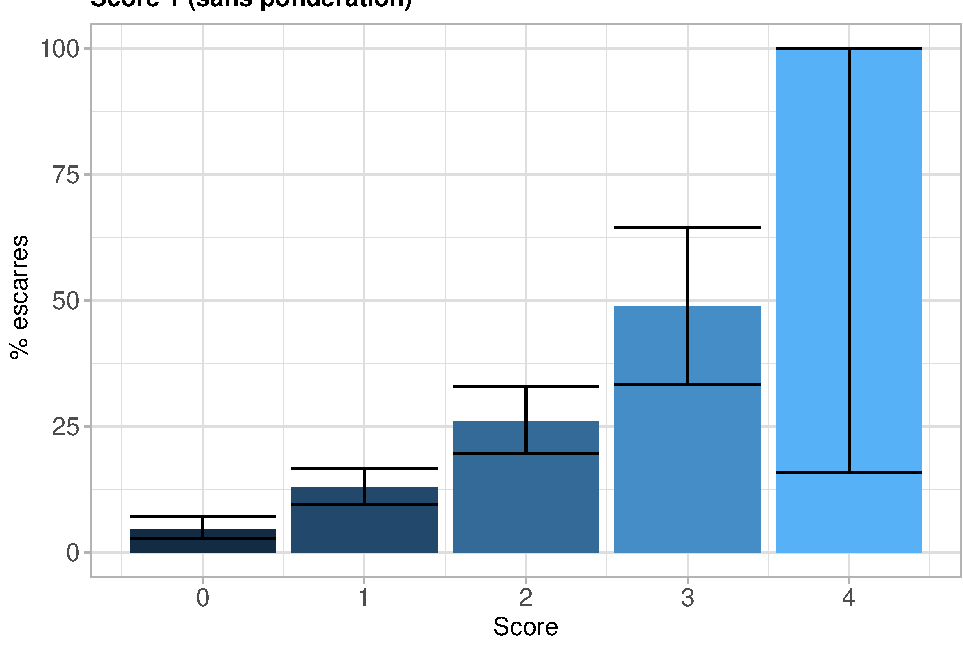
\includegraphics{book_escarre_files/figure-latex/unnamed-chunk-2-1.pdf}


\end{document}
